\documentclass[11pt,a4paper]{article}

\usepackage{geometry}
\usepackage{graphicx, hyperref}
\usepackage[export]{adjustbox}
\usepackage[USenglish]{babel}
\usepackage[utf8]{inputenc}
\usepackage[T1]{fontenc}
\usepackage[usenames,dvipsnames]{color}

\geometry{left=1.5cm, top=0.9cm, right=1.5cm, bottom=1.5cm}

\hypersetup{colorlinks=true,urlcolor=blue}

\begin{document}
    \pagestyle{empty}

    \begin{center}
        \begin{minipage}[b]{3cm}
            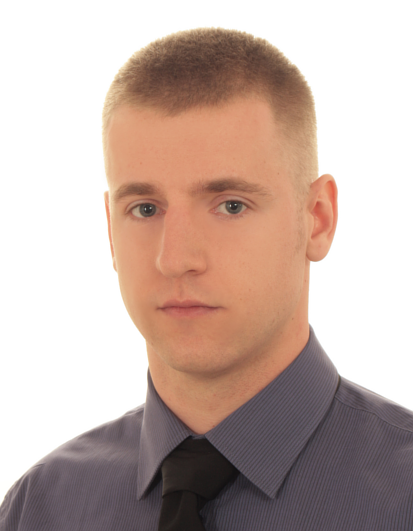
\includegraphics[scale=0.28, right]{photo.png}
        \end{minipage}
        \hspace{0.2cm}
        \begin{minipage}[b]{7cm}
            {\Large \sc Marcin Rainka}
            \begin{description} \itemsep1pt \parskip0pt \parsep0pt
                \item[Address] PCK st. 7/80, 81-621 Gdynia
                \item[Date of birth] 1st December 1989
                \item[Phone number] (+48) 505 464 392
                \item[E-mail] \href{mailto:marcin.rainka@gmail.com}{marcin.rainka@gmail.com}
                \item[LinkedIn] \href{https://linkedin.com/in/marcinrainka}{https://linkedin.com/in/marcinrainka}
            \end{description}
        \end{minipage}
    \end{center}

    \vspace{-0.4cm}

    \noindent\rule{\textwidth}{0.1mm}

    %==================== PROFILE AND OBJECTIVE ====================================================

    \bigskip

    \noindent{\large \bf Profile and objective}

    \smallskip

    \noindent
    Master of~Computer Science with~more than two years of~experience as~a~software developer, familiar with~many technologies, wishing further development and~new challenges.

    %==================== EXPERIENCE ===============================================================

    \bigskip

    \noindent{\large \bf Experience}

    \smallskip

    \noindent{\bf Grupa Wirtualna Polska S.A. -- Junior iOS Developer \hfill September 2016 -- present}
    \vspace{-0.2cm}
    \begin{itemize} \itemsep1pt \parskip0pt \parsep0pt
        \item Developing iOS applications
        \item Writing automated tests
    \end{itemize}
    \vspace{-0.2cm}
    \noindent{\bf AIC S.A. -- Software Developer \hfill April 2014 -- August 2016}
    \vspace{-0.2cm}
    \begin{itemize} \itemsep1pt \parskip0pt \parsep0pt
        \item Developing mobile for~iOS, desktop for~Windows (WPF) and~web applications (AngularJS)
        \item Development of project called iProd, controlling automatic production line with iPads
        \item Creating REST APIs in Python
        \item Writing automated tests and documentation
    \end{itemize}

    %==================== EDUCATION ================================================================

    \medskip
  
    \noindent{\large \bf Education}
  
    \smallskip

    \noindent{{\bf University of Gdańsk}, Faculty of Mathematics, Physics and Informatics \hfill {\bf 2012 -- 2014}}
    \vspace{-0.2cm}
    \begin{itemize} \itemsep1pt \parskip0pt \parsep0pt
        \item[ ] M.Sc in Computer Science degree (daily studies)
    \end{itemize}
    \vspace{-0.2cm}
    \noindent{{\bf University of Warmia and Mazury}, Faculty of Mathematics and Computer Science \hfill {\bf 2008 -- 2012}}
    \vspace{-0.2cm}
    \begin{itemize} \itemsep1pt \parskip0pt \parsep0pt
        \item[ ] B.Eng in Computer Science degree (daily studies)
    \end{itemize}
    \vspace{-0.2cm}
    \noindent{\bf High School No I in Mrągowo \hfill 2005 -- 2008}
    \vspace{-0.2cm}
    \begin{itemize} \itemsep1pt \parskip0pt \parsep0pt
        \item[ ] Mathematics-Physics-Informatics
    \end{itemize}

    %==================== COURSES ==================================================================

    \medskip

    \noindent{\large \bf Additional qualifications}

    \smallskip

    \noindent{Autotesting | Bottega IT Solutions \hfill {\bf April 2015}}

    \noindent{Craftsmanship, patterns and architecture for iOS developers | Bottega IT Solutions \hfill {\bf October 2014}}
  
    %==================== TECHNICAL SKILLS =========================================================

    \bigskip

    \noindent{\large \bf Technical skills}

    %---------- Programming/markup languages -------------------------------------------------------

    \smallskip

    \noindent{\bf Programming/markup languages}

    \smallskip
    $\bullet$ {\bf C\texttt{\#}}
    \hspace{0.34cm}
    $\bullet$ {\bf C\texttt{++}}
    \hspace{0.34cm}
    $\circ$ HTML \& CSS
    \hspace{0.34cm}
    $\circ$ JavaScript
    \hspace{0.34cm}
    $\bullet$ {\bf Objective-C}
    \hspace{0.34cm}
    $\bullet$ {\bf Python}
    \hspace{0.34cm}
    $\circ$ Swift
    \hspace{0.34cm}
    $\circ$ TeX

    %---------- Graphics software ------------------------------------------------------------------

    \smallskip

    \noindent{\bf Graphics software}

    \smallskip
    $\circ$ Blender
    \hspace{0.34cm}
    $\bullet$ {\bf Gimp}
    \hspace{0.34cm}
    $\bullet$ {\bf Inkscape}
    \hspace{0.34cm}
    $\circ$ Sketch

    %---------- Others -----------------------------------------------------------------------------

    \smallskip

    \noindent{\bf Others}

    \smallskip
    $\circ$ AngularJS
    \hspace{0.34cm}
    $\circ$ CUDA
    \hspace{0.34cm}
    $\bullet$ {\bf Flask}
    \hspace{0.34cm}
    $\bullet$ {\bf Git}
    \hspace{0.34cm}
    $\circ$ Jenkins
    \hspace{0.34cm}
    $\circ$ MySQL \& MS SQL

    \vspace{0.04cm}
    $\circ$ Redmine
    \hspace{0.34cm}
    $\circ$ SDL
    \hspace{0.34cm}
    $\circ$ Scrum
    \hspace{0.34cm}
    $\bullet$ {\bf Autotesting}
    \hspace{0.34cm}
    $\bullet$ {\bf WPF}

    %==================== INTERESTS AND HOBBIES ====================================================

    \bigskip

    \noindent{\large \bf Interests and hobbies}

    \smallskip
    $\bullet$ Computer graphics
    \hspace{0.34cm}
    $\bullet$ Drawing and painting
    \hspace{0.34cm}
    $\bullet$ Game development
    \hspace{0.34cm}
    $\bullet$ Powerlifting

    %==================== MISCELLANEOUS ============================================================
  
    \vspace{0.5cm}
    \noindent{\Large \bf Miscellaneous}
  
    \medskip
    \centerline{
        \hfill
        $\bullet$ English B2 (Upper-Intermediate)
        \hfill
        $\bullet$ Driving licence B
        \hfill
    }
  
    %==================== CLAUSE ===================================================================
  
    \vspace{0.92cm}
    \noindent \textit{''I hereby give consent for my personal data to be processed for the~purposes
    of recruitment,\linebreak in accordance with the~Personal Data Protection Act dated 29.08.1997
    (uniform text: Journal of Laws of the~Republic of Poland 2002 No 101, item 926
    with further amendments).''}
\end{document}
